
%(BEGIN_QUESTION)
% Copyright 2012, Tony R. Kuphaldt, released under the Creative Commons Attribution License (v 1.0)
% This means you may do almost anything with this work of mine, so long as you give me proper credit

This control valve is used to control the flow of oil in a refinery unit.  The valve receives a 3-15 PSI signal from an I/P converter, which gets its 4-20 mA signal from a panel-mounted loop controller.  You are tasked with performing a ``live cutover'' of the flow control valve, disconnecting it from the panel-mounted controller and connecting it to a newly installed DCS where operators will be able to control the valve's position from a central control room:

$$\includegraphics[width=15.5cm]{i03395x01.eps}$$

Engineers have already programmed and configured the DCS to control this valve, and technicians have already run a new length of 4-20 mA instrument signal cable from the new DCS to the vicinity of the control valve, waiting to be connected to the I/P.  At the present moment, the control valve is exactly 25\% open.

The challenge is this: the flow through this pipe must not be increased or decreased at all during the cutover -- the flow rate must remain steady during the entire procedure.  Somehow, you must figure out a way to switch the valve's control from the panel-mounted loop controller to the new DCS without affecting the flow of oil through the pipe.

\vskip 10pt

Specify a step-by-step plan to perform this cutover, as though you were giving instructions to another technician.  The only tools and parts you have at your disposal is what is listed below:

\begin{itemize}
\item{} Altek model 334A loop calibrator
\item{} Alligator clip style jumper wires
\item{} Instruction manual for the I/P
\item{} Screwdriver set and combination wrench set (1/4" through 7/8")
\item{} ``Vise-Grip'' style locking pliers
\item{} One medium-size rubber chicken
\end{itemize}


\underbar{file i03395}
%(END_QUESTION)





%(BEGIN_ANSWER)

Possibly the simplest way to do this is to shut the hand valve between the I/P and the control valve's diaphragm (to lock the valve into position), then disconnect the old 4-20 mA cable, then connect the new 4-20 mA cable, then ask the control room operator to set the output to 25\%, then verify the same pressure at the I/P output (as indicated by the gauge) and re-open the hand valve.

\vskip 10pt

Half-credit for any procedure that is unreliable: for instance, relying on split-second timing of connections to avoid valve motion (e.g. ``Connect loop calibrator in source mode at the exact same time you disconnect the loop controller's cable from the I/P'').  Also, doing everything right but not ensuring the DCS is outputting 25\% (like the original controller) before finally cutting it over.

\vskip 10pt

Zero credit if the solution would move the control valve or otherwise alter the flow at all.  For instance, suggesting the loop calibrator be connected to the I/P to drive a certain amount of current, {\it then} the cable disconnected from the loop controller (this would actually drive the valve further open, then return to the original position, as the loop calibrator's current would add to the controller current to form a greater sum through the I/P).

%(END_ANSWER)





%(BEGIN_NOTES)

{\bf This question is intended for exams only and not worksheets!}.

%(END_NOTES)


